\documentclass[12pt,a4paper]{article}
\usepackage[utf8]{inputenc}
\usepackage[vietnamese]{babel}
\usepackage{geometry}
\geometry{top=2cm, bottom=2cm, left=2.5cm, right=2cm}

\usepackage{booktabs}
\usepackage{tabularx}
\usepackage{xltabular}
\usepackage{xcolor}
\usepackage{colortbl}
\usepackage{hyperref}
\usepackage{graphicx}
\usepackage{enumitem}
\usepackage{tcolorbox}
\usepackage{amsmath,amssymb}
\usepackage{fancyhdr}
\usepackage{float}
\usepackage{caption}
\captionsetup[table]{position=top,skip=6pt}
\captionsetup[figure]{position=bottom,skip=6pt}

% Thiết lập màu sắc thương hiệu chuyên nghiệp
\definecolor{brandblue}{RGB}{37, 99, 235}
\definecolor{darkslate}{RGB}{30, 41, 59}
\definecolor{tableheader}{RGB}{239, 246, 255}
\definecolor{lightgray}{RGB}{248, 250, 252}
\definecolor{accentgreen}{RGB}{22, 101, 52}
\definecolor{accentred}{RGB}{153, 27, 27}

% Cấu hình Header & Footer
\pagestyle{fancy}
\fancyhf{}
\setlength{\headheight}{14.5pt}
\fancyhead[L]{\small \textcolor{darkslate}{\textbf{BrewLite} -- Đặc tả Use-Case Trọng Tâm}}
\fancyhead[R]{\small \textcolor{darkslate}{Task 1.3 -- Assignment 2}}
\fancyfoot[C]{\thepage}
\renewcommand{\headrulewidth}{0.4pt}

% Cấu hình liên kết
\hypersetup{
    colorlinks=true,
    linkcolor=brandblue,
    urlcolor=brandblue,
    citecolor=brandblue
}

\begin{document}

% Tiêu đề tài liệu
\begin{center}
    {\LARGE \textbf{\textcolor{brandblue}{ĐẶC TẢ USE-CASE TRỌNG TÂM}}}\\[0.2cm]
    {\large \textbf{UC-01: ĐẶT VÀ THANH TOÁN ĐƠN HÀNG}}\\[0.4cm]
    \begin{tcolorbox}[colback=lightgray,colframe=brandblue,arc=3mm,width=0.96\textwidth]
        \small
        \textbf{Dự án:} Hệ thống Đặt đồ uống trực tuyến BrewLite\\
        \textbf{Học phần:} Công nghệ Phần mềm (Software Engineering) -- Assignment 2\\
        \textbf{Mã nhiệm vụ:} Task 1.3 \hfill \textbf{Mã Use-case:} UC-01\\
        \textbf{Phiên bản:} 1.0 \hfill \textbf{Ngày lập:} 04/11/2026\\
        \textbf{Tệp nguồn PlantUML:} \href{run:../diagrams/usecase-checkout.puml}{\texttt{docs/diagrams/usecase-checkout.puml}}
    \end{tcolorbox}
\end{center}

\vspace{0.2cm}

\section{Giới thiệu \& Bối cảnh nghiệp vụ}
Trong hệ sinh thái ứng dụng đặt đồ uống trực tuyến BrewLite, nghiệp vụ \textbf{``Đặt và thanh toán đơn hàng''} giữ vai trò sống còn (Core Transactional Value). Use-case này kết nối trực tiếp trải nghiệm lựa chọn thức uống của khách hàng (Client Next.js PWA) với hệ thống xử lý giao dịch máy chủ (NestJS API), đảm bảo trừ tồn kho an toàn thông qua cơ chế Khóa lạc quan (Optimistic Concurrency Control), khởi tạo đơn hàng trong cơ chế giao dịch ACID toàn vẹn, và thanh toán chống trừ tiền trùng lặp (Idempotency Key).

\section{Sơ đồ Usecase (Use-Case Diagram)}
\begin{figure}[H]
    \centering
    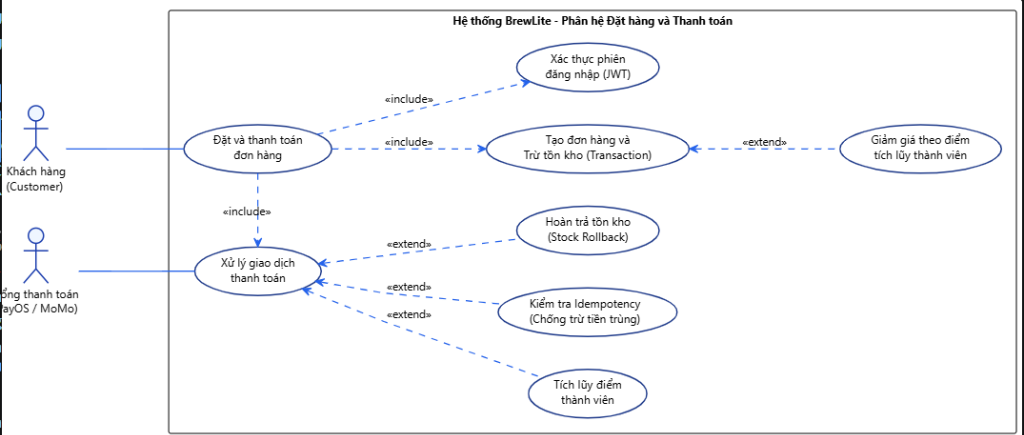
\includegraphics[width=0.95\linewidth]{../diagrams/usecase-checkout.png}
    \caption{Sơ đồ Use-case Đặt và thanh toán đơn hàng}
    \label{fig:usecase-checkout}
\end{figure}

\begin{tcolorbox}[colback=lightgray,colframe=brandblue,arc=2mm,title=\textbf{Cấu trúc quan hệ nghiệp vụ trong sơ đồ:}]
\small
\begin{enumerate}[leftmargin=*,itemsep=2pt]
    \item \textbf{Use-case trọng tâm:} \texttt{Đặt và thanh toán đơn hàng} (Place Order \& Pay)
    \item \textbf{Các Use-case thành phần bắt buộc (\texttt{include}):}
    \begin{itemize}[itemsep=1pt]
        \item \texttt{Xác thực phiên đăng nhập (JWT)}: Kiểm tra tính hợp lệ của token trước khi đặt đơn.
        \item \texttt{Tạo đơn hàng và Trừ tồn kho (Transaction)}: Thực thi trong 1 Database Transaction an toàn.
        \item \texttt{Xử lý giao dịch thanh toán}: Tương tác với Cổng thanh toán (Payment Service) để trừ tiền trong tài khoản.
    \end{itemize}
    \item \textbf{Các Use-case mở rộng theo điều kiện (\texttt{extend}):}
    \begin{itemize}[itemsep=1pt]
        \item \texttt{Giảm giá theo điểm tích lũy thành viên}: \texttt{Đặt và thanh toán đơn hàng} (khi khách đạt hạng Bạc, Vàng, Kim Cương $\ge 20$ điểm).
        \item \texttt{Tích lũy điểm thành viên}: \texttt{Xử lý giao dịch thanh toán} (khi thanh toán thành công chuyển sang \texttt{PAID}).
        \item \texttt{Kiểm tra Idempotency (Chống trừ tiền trùng)}: \texttt{Xử lý giao dịch thanh toán} (khi client gửi lại request cùng key).
        \item \texttt{Hoàn trả tồn kho (Stock Rollback)}: \texttt{Xử lý giao dịch thanh toán} (khi giao dịch bị từ chối / thất bại).
    \end{itemize}
\end{enumerate}
\end{tcolorbox}

\clearpage
\section{Đặc tả chi tiết từng Use-Case}

\subsection{UC-01: Đặt và thanh toán đơn hàng (Use-Case Tổng hợp Trọng tâm)}

\begin{center}
\small
\renewcommand{\arraystretch}{1.2}
\begin{xltabular}{\textwidth}{|>{\bfseries\raggedright\arraybackslash}p{3.2cm}|>{\raggedright\arraybackslash}X|}
\caption{Bảng đặc tả Use-Case chi tiết UC-01: Đặt và thanh toán đơn hàng} \label{tab:uc-01} \\
\hline
\multicolumn{2}{|p{\dimexpr\textwidth-2\tabcolsep-2\arrayrulewidth\relax}|}{\textbf{Usecase ID: UC-01 -- Đặt và thanh toán đơn hàng}} \\
\hline
\multicolumn{2}{|p{\dimexpr\textwidth-2\tabcolsep-2\arrayrulewidth\relax}|}{\textbf{Tóm tắt:} Chức năng cho phép Khách hàng kiểm tra giỏ hàng, áp dụng giảm giá dựa trên điểm tích lũy thành viên, kiểm tra và trừ tồn kho bằng Database Transaction an toàn, thực hiện thanh toán qua Cổng thanh toán (hỗ trợ Idempotency chống trừ tiền trùng) và tích lũy điểm thưởng thành viên khi hoàn tất.} \\
\hline
\endfirsthead

\hline
\multicolumn{2}{|p{\dimexpr\textwidth-2\tabcolsep-2\arrayrulewidth\relax}|}{\textbf{Usecase ID: UC-01 -- Đặt và thanh toán đơn hàng (tiếp theo)}} \\
\hline
\endhead

\hline
\multicolumn{2}{|r|}{\small\textit{(Xem tiếp trang sau...)}} \\
\hline
\endfoot

\hline
\endlastfoot

Dòng sự kiện chính & 
\begin{enumerate}[leftmargin=*,itemsep=2pt,topsep=2pt,parsep=0pt,partopsep=0pt]
    \item Khách hàng (Customer) truy cập giỏ hàng trên Giao diện người dùng (Next.js UI) và nhấn nút \textbf{``Tiến hành đặt hàng''}.
    \item Next.js UI gửi yêu cầu xác thực phiên đăng nhập (JWT Bearer Token) đến Hệ thống Backend (NestJS API).
    \item NestJS API xác thực tính hợp lệ của Token, trích xuất mã người dùng (\texttt{userId}) cùng số điểm tích lũy thành viên (\texttt{loyaltyPoints}) hiện có.
    \item Next.js UI tính toán chiết khấu giảm giá thành viên, hiển thị tổng tiền cuối cùng và Khách hàng nhấn \textbf{``Xác nhận thanh toán''}.
    \item Next.js UI sinh mã khóa Idempotency độc nhất (\texttt{idempotencyKey}) và gửi yêu cầu tạo đơn hàng \texttt{POST /orders} kèm chi tiết giỏ hàng đến NestJS API.
    \item NestJS API mở Transaction (\texttt{\$transaction}) trên Cơ sở dữ liệu (PostgreSQL): kiểm tra tồn kho (\texttt{stock >= quantity}), trừ kho theo khóa lạc quan (\texttt{version}), áp dụng giảm giá điểm tích lũy và lưu bản ghi Đơn hàng với trạng thái \texttt{PENDING}.
    \item Next.js UI nhận phản hồi tạo đơn thành công, tiếp tục gửi yêu cầu xử lý thanh toán \texttt{POST /payments} kèm \texttt{orderId}, phương thức thanh toán và \texttt{idempotencyKey} đến NestJS API.
    \item NestJS API kiểm tra khóa \texttt{idempotencyKey} trong CSDL chống trùng lặp, sau đó chuyển tiếp yêu cầu giao dịch sang Cổng thanh toán (PayOS / MoMo).
    \item Cổng thanh toán xử lý trừ tiền từ tài khoản/ví của khách hàng và phản hồi trạng thái \texttt{SUCCESS} kèm mã giao dịch (\texttt{transactionId}) về cho NestJS API.
    \item NestJS API mở Database Transaction: cập nhật trạng thái đơn hàng sang \texttt{PAID}, lưu bản ghi thanh toán, tự động cộng điểm tích lũy thành viên cho khách hàng, và phản hồi HTTP \texttt{200 OK}.
    \item Next.js UI nhận kết quả thành công, thực hiện xóa sạch giỏ hàng (\texttt{clearCart()}) và điều hướng khách hàng đến màn hình chi tiết theo dõi đơn hàng (\texttt{/orders/:id}).
\end{enumerate} \\
\hline
Dòng sự kiện phụ & 
\begin{itemize}[leftmargin=*,itemsep=2pt,topsep=2pt,parsep=0pt,partopsep=0pt]
    \item \textbf{2a. Phiên đăng nhập hết hạn hoặc chưa đăng nhập:} Next.js UI lưu trạng thái giỏ hàng và chuyển hướng người dùng đến trang Đăng nhập (\texttt{/login?redirect=/checkout}).
    \item \textbf{4a. Khách hàng chưa đạt mốc tích lũy điểm:} Hệ thống không áp dụng chiết khấu, giữ nguyên giá gốc của đơn hàng.
    \item \textbf{6a. Sản phẩm hết hàng hoặc xung đột tồn kho (Optimistic Lock):} NestJS API hủy bỏ Transaction (Rollback $100\%$) và trả về HTTP 400/409; Next.js UI hiển thị thông báo lỗi để người dùng điều chỉnh lại giỏ hàng.
    \item \textbf{8a. Gửi lại request với Idempotency Key đã tồn tại:} NestJS API phát hiện khóa đã được xử lý thành công, lập tức trả về kết quả cũ kèm HTTP 200 mà không gọi Cổng thanh toán lần 2 (ngăn chặn trừ tiền trùng).
    \item \textbf{9a. Cổng thanh toán từ chối hoặc giao dịch thất bại:} Cổng thanh toán trả về \texttt{FAILED}; NestJS API cập nhật trạng thái đơn thành \texttt{PAYMENT\_FAILED}, kích hoạt cơ chế hoàn trả số lượng kho đã trừ (Stock Rollback) và báo lỗi về UI để khách thử lại phương thức khác.
    \item \textbf{9b. Cổng thanh toán mất kết nối hoặc quá thời gian (Timeout):} NestJS API giữ đơn hàng ở trạng thái \texttt{PENDING} để phục vụ cơ chế đối soát hoặc kiểm tra lại sau.
\end{itemize} \\
\hline
Tiền điều kiện & 
\begin{itemize}[leftmargin=*,itemsep=2pt,topsep=2pt,parsep=0pt,partopsep=0pt]
    \item Khách hàng đã đăng nhập vào hệ thống và sở hữu JSON Web Token (JWT Bearer) còn hiệu lực.
    \item Giỏ hàng có ít nhất một sản phẩm hợp lệ (\texttt{items.length > 0}).
    \item Toàn bộ sản phẩm và topping trong đơn hàng đều đang được mở bán (\texttt{isAvailable = true}).
\end{itemize} \\
\hline
Hậu điều kiện & 
\begin{itemize}[leftmargin=*,itemsep=2pt,topsep=2pt,parsep=0pt,partopsep=0pt]
    \item \textbf{Hậu điều kiện thành công (Success):} Đơn hàng được lưu vào CSDL với trạng thái \texttt{PAID}; tồn kho bị trừ tương ứng và trường \texttt{version} tăng 1; giao dịch thanh toán được ghi nhận cùng \texttt{idempotencyKey}; khách hàng được cộng điểm tích lũy thành viên; giỏ hàng được làm rỗng và giao diện chuyển đến trang chi tiết đơn hàng.
    \item \textbf{Hậu điều kiện thất bại (Failure):} Giao dịch bị Rollback hoặc được hoàn trả tồn kho (Stock Rollback); đơn hàng chuyển sang trạng thái \texttt{PAYMENT\_FAILED} hoặc không được tạo; giỏ hàng của khách hàng được bảo lưu nguyên vẹn.
\end{itemize} \\
\hline
\end{xltabular}
\end{center}

\subsection{UC-02: Xác thực phiên đăng nhập (JWT)}

\begin{table}[H]
\centering
\small
\renewcommand{\arraystretch}{1.2}
\begin{tabularx}{\textwidth}{|>{\bfseries\raggedright\arraybackslash}p{3.2cm}|>{\raggedright\arraybackslash}X|}
\hline
\multicolumn{2}{|p{\dimexpr\textwidth-2\tabcolsep-2\arrayrulewidth\relax}|}{\textbf{Usecase ID: UC-02 -- Xác thực phiên đăng nhập (JWT)}} \\
\hline
\multicolumn{2}{|p{\dimexpr\textwidth-2\tabcolsep-2\arrayrulewidth\relax}|}{\textbf{Tóm tắt:} Chức năng kiểm tra tính hợp lệ và thời hạn của JSON Web Token (JWT Bearer) trong request header nhằm xác thực danh tính khách hàng trước khi cho phép thực hiện các thao tác đặt hàng và thanh toán.} \\
\hline
Dòng sự kiện chính & 
\begin{enumerate}[leftmargin=*,itemsep=2pt,topsep=2pt,parsep=0pt,partopsep=0pt]
    \item Next.js UI lấy chuỗi Bearer Token từ bộ nhớ LocalStorage và đính kèm vào Header \texttt{Authorization: Bearer <token>} của HTTP request.
    \item Next.js UI gửi request đến NestJS API.
    \item \texttt{AuthGuard} tại NestJS API chặn request và trích xuất chuỗi token từ Header.
    \item \texttt{JwtService} thực hiện giải mã (verify signature) bằng secret key của hệ thống và kiểm tra thời hạn sống (\texttt{exp}) của token.
    \item Hệ thống trích xuất thông tin người dùng (\texttt{userId}, \texttt{role}, \texttt{email}) và gán vào context đối tượng \texttt{Request.user}.
    \item NestJS API cho phép request tiếp tục đi vào controller xử lý đơn hàng.
\end{enumerate} \\
\hline
Dòng sự kiện phụ & 
\begin{itemize}[leftmargin=*,itemsep=2pt,topsep=2pt,parsep=0pt,partopsep=0pt]
    \item \textbf{1a. Token không tồn tại (chưa đăng nhập):} Next.js UI chuyển hướng người dùng sang trang Đăng nhập (\texttt{/login?redirect=/checkout}).
    \item \textbf{4a. Token không hợp lệ hoặc bị giả mạo:} NestJS API từ chối request và trả về mã lỗi HTTP 401 Unauthorized.
    \item \textbf{4b. Token đã hết hạn (Expired Token):} NestJS API trả về HTTP 401; UI xóa token cũ trong LocalStorage và yêu cầu khách hàng đăng nhập lại.
\end{itemize} \\
\hline
Tiền điều kiện & Khách hàng thực hiện hành động yêu cầu định danh (xác nhận giỏ hàng, đặt hàng, gửi thanh toán). \\
\hline
Hậu điều kiện & 
\begin{itemize}[leftmargin=*,itemsep=2pt,topsep=2pt,parsep=0pt,partopsep=0pt]
    \item \textbf{Thành công:} Danh tính khách hàng được xác thực hợp lệ và gán vào request context, cho phép thực thi logic nghiệp vụ tiếp theo.
    \item \textbf{Thất bại:} Request bị chặn lại với mã lỗi HTTP 401 Unauthorized, không có dữ liệu nghiệp vụ nào bị sửa đổi.
\end{itemize} \\
\hline
\end{tabularx}
\caption{Bảng đặc tả Use-Case UC-02: Xác thực phiên đăng nhập (JWT)}
\label{tab:uc-02}
\end{table}

\subsection{UC-03: Tạo đơn hàng và Trừ tồn kho (Transaction)}

\begin{table}[H]
\centering
\small
\renewcommand{\arraystretch}{1.2}
\begin{tabularx}{\textwidth}{|>{\bfseries\raggedright\arraybackslash}p{3.2cm}|>{\raggedright\arraybackslash}X|}
\hline
\multicolumn{2}{|p{\dimexpr\textwidth-2\tabcolsep-2\arrayrulewidth\relax}|}{\textbf{Usecase ID: UC-03 -- Tạo đơn hàng và Trừ tồn kho (Transaction)}} \\
\hline
\multicolumn{2}{|p{\dimexpr\textwidth-2\tabcolsep-2\arrayrulewidth\relax}|}{\textbf{Tóm tắt:} Chức năng khởi tạo bản ghi đơn hàng ở trạng thái \texttt{PENDING} và đồng thời trừ số lượng tồn kho theo cơ chế Khóa lạc quan (Optimistic Concurrency Control qua trường \texttt{version}) trong một Atomic Database Transaction an toàn.} \\
\hline
Dòng sự kiện chính & 
\begin{enumerate}[leftmargin=*,itemsep=2pt,topsep=2pt,parsep=0pt,partopsep=0pt]
    \item Next.js UI gửi request \texttt{POST /orders} kèm chi tiết giỏ hàng và Bearer JWT Token đến NestJS API.
    \item NestJS API kiểm tra trạng thái mở bán (\texttt{isAvailable = true}) của các sản phẩm và topping trong đơn hàng.
    \item NestJS API mở Transaction nguyên tử trên PostgreSQL (\texttt{prisma.\$transaction}).
    \item Hệ thống truy vấn tồn kho hiện tại và số phiên bản \texttt{version} của từng sản phẩm trong giỏ hàng.
    \item Hệ thống kiểm tra số lượng khả dụng: nếu \texttt{stock >= requestedQuantity}, thực hiện trừ tồn kho và tăng phiên bản (\texttt{stock = stock - qty}, \texttt{version = version + 1}).
    \item Hệ thống tạo bản ghi \texttt{Order} với trạng thái \texttt{PENDING}, cùng các bản ghi con \texttt{OrderItem} và \texttt{OrderItemTopping}.
    \item Database Transaction commit thành công; NestJS API phản hồi HTTP 201 Created kèm \texttt{orderId} và \texttt{totalAmount}.
\end{enumerate} \\
\hline
Dòng sự kiện phụ & 
\begin{itemize}[leftmargin=*,itemsep=2pt,topsep=2pt,parsep=0pt,partopsep=0pt]
    \item \textbf{5a. Tồn kho không đủ (\texttt{stock < qty}):} Transaction tự động Rollback $100\%$, API trả về HTTP 400 Bad Request kèm thông báo sản phẩm đã hết hàng.
    \item \textbf{5b. Xung đột ghi đồng thời (Optimistic Lock -- sai \texttt{version}):} Transaction Rollback, trả về HTTP 409 Conflict yêu cầu khách hàng thử lại.
\end{itemize} \\
\hline
Tiền điều kiện & Khách hàng đã được xác thực danh tính (JWT hợp lệ); giỏ hàng có ít nhất một sản phẩm mở bán. \\
\hline
Hậu điều kiện & 
\begin{itemize}[leftmargin=*,itemsep=2pt,topsep=2pt,parsep=0pt,partopsep=0pt]
    \item \textbf{Thành công:} Đơn hàng mới được tạo ở trạng thái \texttt{PENDING}; tồn kho sản phẩm bị trừ chính xác và \texttt{version} tăng thêm 1.
    \item \textbf{Thất bại:} CSDL giữ nguyên trạng thái ban đầu, không phát sinh đơn hàng rác và tồn kho không bị trừ âm.
\end{itemize} \\
\hline
\end{tabularx}
\caption{Bảng đặc tả Use-Case UC-03: Tạo đơn hàng và Trừ tồn kho (Transaction)}
\label{tab:uc-03}
\end{table}

\subsection{UC-04: Giảm giá theo điểm tích lũy thành viên}

\begin{table}[H]
\centering
\small
\renewcommand{\arraystretch}{1.2}
\begin{tabularx}{\textwidth}{|>{\bfseries\raggedright\arraybackslash}p{3.2cm}|>{\raggedright\arraybackslash}X|}
\hline
\multicolumn{2}{|p{\dimexpr\textwidth-2\tabcolsep-2\arrayrulewidth\relax}|}{\textbf{Usecase ID: UC-04 -- Giảm giá theo điểm tích lũy thành viên}} \\
\hline
\multicolumn{2}{|p{\dimexpr\textwidth-2\tabcolsep-2\arrayrulewidth\relax}|}{\textbf{Tóm tắt:} Chức năng tự động xác định mức chiết khấu phần trăm trên tổng giá trị đơn hàng dựa trên số điểm tích lũy và hạng thành viên của khách hàng (Bạc $\ge 20$ điểm: 5\%, Vàng $\ge 50$ điểm: 10\%, Kim Cương $\ge 100$ điểm: 15\%).} \\
\hline
Dòng sự kiện chính & 
\begin{enumerate}[leftmargin=*,itemsep=2pt,topsep=2pt,parsep=0pt,partopsep=0pt]
    \item Trong quá trình tính toán giá trị đơn hàng, NestJS API truy vấn điểm tích lũy (\texttt{loyaltyPoints}) của khách hàng từ bảng \texttt{User}.
    \item Hệ thống đối chiếu điểm số với các mốc xếp hạng thành viên:
    \begin{itemize}[itemsep=1pt]
        \item Dưới 20 điểm (Hạng Chuẩn): Chiết khấu 0\%.
        \item Từ 20 đến 49 điểm (Hạng Bạc): Chiết khấu 5\% tổng tiền món.
        \item Từ 50 đến 99 điểm (Hạng Vàng): Chiết khấu 10\% tổng tiền món.
        \item Từ 100 điểm trở lên (Hạng Kim Cương): Chiết khấu 15\% tổng tiền món.
    \end{itemize}
    \item Hệ thống tính số tiền giảm giá (\texttt{discountAmount}) và tính lại tổng tiền thanh toán: \texttt{finalAmount = totalAmount - discountAmount}.
    \item Hệ thống lưu giá trị chiết khấu vào đơn hàng và phản hồi về cho Next.js UI hiển thị chi tiết số tiền được giảm cho khách hàng.
\end{enumerate} \\
\hline
Dòng sự kiện phụ & 
\begin{itemize}[leftmargin=*,itemsep=2pt,topsep=2pt,parsep=0pt,partopsep=0pt]
    \item \textbf{2a. Khách hàng chưa đạt mốc 20 điểm:} Không áp dụng chiết khấu (\texttt{discountAmount = 0}), tổng tiền thanh toán giữ nguyên giá gốc.
    \item \textbf{3a. Lỗi truy xuất điểm tích lũy:} Hệ thống mặc định tính theo giá gốc để không gián đoạn quy trình đặt hàng của khách.
\end{itemize} \\
\hline
Tiền điều kiện & Khách hàng đã đăng nhập và đang trong bước tính giá trị đơn hàng; thỏa mãn điều kiện điểm tích lũy $\ge 20$. \\
\hline
Hậu điều kiện & 
\begin{itemize}[leftmargin=*,itemsep=2pt,topsep=2pt,parsep=0pt,partopsep=0pt]
    \item \textbf{Thành công:} Tổng số tiền khách hàng cần thanh toán được giảm trừ chính xác theo tỷ lệ chiết khấu của hạng thành viên.
    \item \textbf{Thất bại:} Không áp dụng chiết khấu, đơn hàng giữ nguyên giá trị niêm yết ban đầu.
\end{itemize} \\
\hline
\end{tabularx}
\caption{Bảng đặc tả Use-Case UC-04: Giảm giá theo điểm tích lũy thành viên}
\label{tab:uc-04}
\end{table}

\subsection{UC-05: Xử lý giao dịch thanh toán}

\begin{table}[H]
\centering
\small
\renewcommand{\arraystretch}{1.2}
\begin{tabularx}{\textwidth}{|>{\bfseries\raggedright\arraybackslash}p{3.2cm}|>{\raggedright\arraybackslash}X|}
\hline
\multicolumn{2}{|p{\dimexpr\textwidth-2\tabcolsep-2\arrayrulewidth\relax}|}{\textbf{Usecase ID: UC-05 -- Xử lý giao dịch thanh toán}} \\
\hline
\multicolumn{2}{|p{\dimexpr\textwidth-2\tabcolsep-2\arrayrulewidth\relax}|}{\textbf{Tóm tắt:} Chức năng tiếp nhận yêu cầu thanh toán cho đơn hàng đã tạo, kiểm tra Idempotency, chuyển tiếp giao dịch sang Cổng thanh toán (PayOS / MoMo), cập nhật trạng thái đơn hàng sang \texttt{PAID} và kích hoạt tích lũy điểm khi thành công.} \\
\hline
Dòng sự kiện chính & 
\begin{enumerate}[leftmargin=*,itemsep=2pt,topsep=2pt,parsep=0pt,partopsep=0pt]
    \item Next.js UI gửi yêu cầu \texttt{POST /payments} kèm \texttt{orderId}, phương thức thanh toán (\texttt{WALLET}/\texttt{CARD}), \texttt{amount} và \texttt{idempotencyKey} đến NestJS API.
    \item NestJS API kiểm tra trạng thái đơn hàng trong CSDL (phải là \texttt{PENDING}).
    \item Kích hoạt use-case kiểm tra Idempotency để xác minh giao dịch chưa từng được thực hiện.
    \item NestJS API gửi yêu cầu trừ tiền sang API Cổng thanh toán (PayOS / MoMo).
    \item Cổng thanh toán xác thực số dư tài khoản/ví, thực hiện trừ tiền và phản hồi trạng thái \texttt{SUCCESS} kèm \texttt{transactionId}.
    \item NestJS API mở Transaction cập nhật trạng thái đơn hàng thành \texttt{PAID}, tạo bản ghi \texttt{Payment} thành công.
    \item Kích hoạt use-case tích lũy điểm thành viên cho khách hàng.
    \item NestJS API phản hồi HTTP 200 OK để Next.js UI thông báo thành công và làm rỗng giỏ hàng.
\end{enumerate} \\
\hline
Dòng sự kiện phụ & 
\begin{itemize}[leftmargin=*,itemsep=2pt,topsep=2pt,parsep=0pt,partopsep=0pt]
    \item \textbf{2a. Đơn hàng không tồn tại hoặc đã được thanh toán trước đó:} NestJS API từ chối và trả về HTTP 400 Bad Request.
    \item \textbf{5a. Cổng thanh toán từ chối hoặc giao dịch thất bại (Ví không đủ tiền, lỗi thẻ):} Cổng thanh toán phản hồi \texttt{FAILED} $\rightarrow$ Kích hoạt use-case Hoàn trả tồn kho (Stock Rollback), đơn hàng chuyển sang \texttt{PAYMENT\_FAILED}.
    \item \textbf{5b. Cổng thanh toán mất kết nối hoặc quá thời gian (Timeout):} Giữ nguyên trạng thái đơn hàng là \texttt{PENDING} để phục vụ cơ chế đối soát sau.
\end{itemize} \\
\hline
Tiền điều kiện & Đơn hàng đã được tạo thành công ở trạng thái \texttt{PENDING}; có chuỗi \texttt{idempotencyKey} duy nhất. \\
\hline
Hậu điều kiện & 
\begin{itemize}[leftmargin=*,itemsep=2pt,topsep=2pt,parsep=0pt,partopsep=0pt]
    \item \textbf{Thành công:} Đơn hàng chuyển sang \texttt{PAID}, bản ghi thanh toán được lưu trữ, điểm thưởng được cộng cho khách hàng.
    \item \textbf{Thất bại:} Đơn hàng chuyển sang \texttt{PAYMENT\_FAILED}, tồn kho được hoàn trả lại đầy đủ, khách hàng nhận thông báo thử lại.
\end{itemize} \\
\hline
\end{tabularx}
\caption{Bảng đặc tả Use-Case UC-05: Xử lý giao dịch thanh toán}
\label{tab:uc-05}
\end{table}

\subsection{UC-06: Kiểm tra Idempotency (Chống trừ tiền trùng)}

\begin{table}[H]
\centering
\small
\renewcommand{\arraystretch}{1.2}
\begin{tabularx}{\textwidth}{|>{\bfseries\raggedright\arraybackslash}p{3.2cm}|>{\raggedright\arraybackslash}X|}
\hline
\multicolumn{2}{|p{\dimexpr\textwidth-2\tabcolsep-2\arrayrulewidth\relax}|}{\textbf{Usecase ID: UC-06 -- Kiểm tra Idempotency (Chống trừ tiền trùng)}} \\
\hline
\multicolumn{2}{|p{\dimexpr\textwidth-2\tabcolsep-2\arrayrulewidth\relax}|}{\textbf{Tóm tắt:} Chức năng kiểm tra tính duy nhất của mã khóa Idempotency trong CSDL trước khi thực hiện giao dịch tài chính, ngăn chặn tình trạng khách hàng bị trừ tiền hai lần khi mạng lag hoặc bấm gửi nhiều lần.} \\
\hline
Dòng sự kiện chính & 
\begin{enumerate}[leftmargin=*,itemsep=2pt,topsep=2pt,parsep=0pt,partopsep=0pt]
    \item PaymentsService tiếp nhận chuỗi \texttt{idempotencyKey} từ request thanh toán của Client.
    \item Hệ thống thực hiện truy vấn bảng \texttt{Payment} trong PostgreSQL theo trường \texttt{idempotencyKey}.
    \item Nếu khóa \textbf{chưa} tồn tại trong CSDL: Hệ thống ghi nhận khóa này và cho phép tiếp tục quy trình gọi sang Cổng thanh toán.
\end{enumerate} \\
\hline
Dòng sự kiện phụ & 
\begin{itemize}[leftmargin=*,itemsep=2pt,topsep=2pt,parsep=0pt,partopsep=0pt]
    \item \textbf{3a. Khóa đã tồn tại với trạng thái \texttt{COMPLETED}:}
    \begin{enumerate}[itemsep=1pt]
        \item Hệ thống nhận diện đây là yêu cầu gửi lại (retry do mạng lag).
        \item Hệ thống lập tức ngắt luồng gọi sang Cổng thanh toán (chặn hoàn toàn việc trừ tiền lần 2).
        \item Hệ thống lấy dữ liệu kết quả thanh toán trước đó trong CSDL và phản hồi ngay HTTP 200 OK kèm thông tin giao dịch cũ.
    \end{enumerate}
    \item \textbf{3b. Khóa đã tồn tại với trạng thái \texttt{PROCESSING}:} Hệ thống trả về HTTP 409 Conflict thông báo giao dịch đang được xử lý, đề nghị khách hàng chờ kết quả.
\end{itemize} \\
\hline
Tiền điều kiện & Yêu cầu thanh toán gửi đến hệ thống có đính kèm tham số \texttt{idempotencyKey}. \\
\hline
Hậu điều kiện & 
\begin{itemize}[leftmargin=*,itemsep=2pt,topsep=2pt,parsep=0pt,partopsep=0pt]
    \item \textbf{Thành công:} Đảm bảo giao dịch chỉ được trừ tiền duy nhất một lần trên Cổng thanh toán bất kể số lần Client gửi lại request.
    \item \textbf{Thất bại:} Không có giao dịch trùng lặp nào được tạo trong hệ thống.
\end{itemize} \\
\hline
\end{tabularx}
\caption{Bảng đặc tả Use-Case UC-06: Kiểm tra Idempotency (Chống trừ tiền trùng)}
\label{tab:uc-06}
\end{table}

\subsection{UC-07: Hoàn trả tồn kho (Stock Rollback)}

\begin{table}[H]
\centering
\small
\renewcommand{\arraystretch}{1.2}
\begin{tabularx}{\textwidth}{|>{\bfseries\raggedright\arraybackslash}p{3.2cm}|>{\raggedright\arraybackslash}X|}
\hline
\multicolumn{2}{|p{\dimexpr\textwidth-2\tabcolsep-2\arrayrulewidth\relax}|}{\textbf{Usecase ID: UC-07 -- Hoàn trả tồn kho (Stock Rollback)}} \\
\hline
\multicolumn{2}{|p{\dimexpr\textwidth-2\tabcolsep-2\arrayrulewidth\relax}|}{\textbf{Tóm tắt:} Chức năng tự động cộng bù lại số lượng tồn kho của các sản phẩm đã tạm trừ trước đó khi giao dịch thanh toán bị từ chối hoặc thất bại, giải phóng hàng tồn ảo cho các khách hàng khác đặt mua.} \\
\hline
Dòng sự kiện chính & 
\begin{enumerate}[leftmargin=*,itemsep=2pt,topsep=2pt,parsep=0pt,partopsep=0pt]
    \item Khi nhận tín hiệu thanh toán thất bại (\texttt{FAILED}) từ Cổng thanh toán hoặc lỗi hệ thống:
    \item NestJS API mở Transaction nguyên tử trong PostgreSQL.
    \item Cập nhật trạng thái của đơn hàng \texttt{Order} sang \texttt{PAYMENT\_FAILED}.
    \item Hệ thống truy vấn danh sách các món và số lượng mua tương ứng từ bảng \texttt{OrderItem}.
    \item Với từng sản phẩm, hệ thống thực hiện hoàn kho: \texttt{stock = stock + quantity}, đồng thời tăng \texttt{version = version + 1}.
    \item Hệ thống commit Transaction hoàn kho và ghi log kiểm toán sự kiện (Audit Log: Stock Rollback Completed).
    \item Phản hồi thông báo lỗi về Next.js UI để khách hàng có thể chọn phương thức thanh toán khác hoặc đặt lại.
\end{enumerate} \\
\hline
Dòng sự kiện phụ & 
\begin{itemize}[leftmargin=*,itemsep=2pt,topsep=2pt,parsep=0pt,partopsep=0pt]
    \item \textbf{4a. Không tìm thấy chi tiết món trong đơn hàng:} Hệ thống phát tín hiệu cảnh báo khẩn cấp (Critical Log) để quản trị viên kiểm tra dữ liệu thủ công.
\end{itemize} \\
\hline
Tiền điều kiện & Đơn hàng đã trừ kho trước đó nhưng giao dịch thanh toán bị hủy, từ chối hoặc thất bại. \\
\hline
Hậu điều kiện & 
\begin{itemize}[leftmargin=*,itemsep=2pt,topsep=2pt,parsep=0pt,partopsep=0pt]
    \item \textbf{Thành công:} Toàn bộ số lượng sản phẩm được hoàn trả chính xác vào kho hàng; trạng thái đơn hàng là \texttt{PAYMENT\_FAILED}.
    \item \textbf{Thất bại:} Transaction hoàn kho được tự động thử lại (retry queue) để đảm bảo không bị thất thoát hàng hóa.
\end{itemize} \\
\hline
\end{tabularx}
\caption{Bảng đặc tả Use-Case UC-07: Hoàn trả tồn kho (Stock Rollback)}
\label{tab:uc-07}
\end{table}

\subsection{UC-08: Tích lũy điểm thành viên}

\begin{table}[H]
\centering
\small
\renewcommand{\arraystretch}{1.2}
\begin{tabularx}{\textwidth}{|>{\bfseries\raggedright\arraybackslash}p{3.2cm}|>{\raggedright\arraybackslash}X|}
\hline
\multicolumn{2}{|p{\dimexpr\textwidth-2\tabcolsep-2\arrayrulewidth\relax}|}{\textbf{Usecase ID: UC-08 -- Tích lũy điểm thành viên}} \\
\hline
\multicolumn{2}{|p{\dimexpr\textwidth-2\tabcolsep-2\arrayrulewidth\relax}|}{\textbf{Tóm tắt:} Chức năng tính toán và tự động cộng điểm thưởng tích lũy vào tài khoản khách hàng sau khi đơn hàng được thanh toán thành công ($10.000\text{ VNĐ} = 1\text{ điểm}$).} \\
\hline
Dòng sự kiện chính & 
\begin{enumerate}[leftmargin=*,itemsep=2pt,topsep=2pt,parsep=0pt,partopsep=0pt]
    \item Sau khi Cổng thanh toán phản hồi \texttt{SUCCESS} và đơn hàng chuyển sang \texttt{PAID}:
    \item NestJS API lấy giá trị thanh toán thực tế (\texttt{totalAmount}) của đơn hàng.
    \item Hệ thống tính số điểm thưởng tích lũy: \texttt{points = floor(totalAmount / 10000)}.
    \item NestJS API mở Transaction cộng điểm vào trường \texttt{loyaltyPoints} của người dùng trong bảng \texttt{User}: \texttt{loyaltyPoints = loyaltyPoints + points}.
    \item Hệ thống ghi lại bản ghi lịch sử cộng điểm vào bảng lưu vết (Loyalty History).
    \item Phản hồi số điểm mới tích lũy về Next.js UI để hiển thị thông báo chúc mừng trên màn hình thành công.
\end{enumerate} \\
\hline
Dòng sự kiện phụ & 
\begin{itemize}[leftmargin=*,itemsep=2pt,topsep=2pt,parsep=0pt,partopsep=0pt]
    \item \textbf{3a. Tổng tiền đơn hàng dưới 10.000 VNĐ:} Số điểm tích lũy cộng thêm là 0 điểm.
    \item \textbf{4a. Gặp lỗi khi cộng điểm vào CSDL:} Không làm gián đoạn trạng thái đơn hàng (đơn hàng vẫn là \texttt{PAID}), tác vụ cộng điểm được đẩy vào hàng đợi retry để xử lý lại.
\end{itemize} \\
\hline
Tiền điều kiện & Đơn hàng đã được thanh toán thành công và chuyển sang trạng thái \texttt{PAID}. \\
\hline
Hậu điều kiện & 
\begin{itemize}[leftmargin=*,itemsep=2pt,topsep=2pt,parsep=0pt,partopsep=0pt]
    \item \textbf{Thành công:} Điểm thưởng của khách hàng được cập nhật tăng thêm tương ứng, khách hàng có thể dùng điểm để nâng hạng và nhận chiết khấu cho các đơn hàng tiếp theo.
    \item \textbf{Thất bại:} Không ảnh hưởng đến đơn hàng đã thanh toán thành công.
\end{itemize} \\
\hline
\end{tabularx}
\caption{Bảng đặc tả Use-Case UC-08: Tích lũy điểm thành viên}
\label{tab:uc-08}
\end{table}

\section{Phạm vi hệ thống: Hệ thống Làm gì và Không làm gì}

\begin{table}[H]
\centering
\small
\begin{tabularx}{\textwidth}{>{\raggedright\arraybackslash}p{7.5cm} >{\raggedright\arraybackslash}X}
\toprule
\rowcolor{tableheader}
\textbf{Hệ thống LÀM GÌ (In-Scope System Behaviors)} & \textbf{Hệ thống KHÔNG LÀM GÌ (Out-of-Scope)} \\
\midrule
Xác thực danh tính người dùng bằng JWT Token trước khi cho phép đặt hàng và thanh toán. & \textbf{Không} hỗ trợ thanh toán nặc danh (guest checkout) thiếu tài khoản định danh. \\
\addlinespace
Kiểm soát tồn kho tức thời bằng Khóa lạc quan (Optimistic Concurrency Control qua trường \texttt{version}) ngăn chặn bán âm kho (Overselling). & \textbf{Không} khóa giữ hàng tồn kho vĩnh viễn trong giỏ khi khách chưa tiến hành bấm thanh toán. \\
\addlinespace
Thực thi toàn bộ quy trình tạo đơn, chi tiết món và trừ kho trong một Atomic Transaction (\texttt{\$transaction}) duy nhất. & \textbf{Không} tách rời việc trừ kho và tạo đơn thành các bước riêng rẽ ngoài transaction. \\
\addlinespace
Chống trừ tiền trùng lặp thông qua cơ chế \texttt{idempotencyKey}. Nếu gửi lại cùng một key, trả về kết quả cũ mà không trừ tiền lần 2. & \textbf{Không} tích hợp cổng thanh toán thực tế phức tạp (chỉ dùng Payment Gateway mô phỏng chuẩn giao thức). \\
\addlinespace
Tự động tính và cộng điểm tích lũy thành viên (\texttt{loyaltyPoints}) ngay khi thanh toán thành công. & \textbf{Không} xử lý phân hệ vận chuyển giao hàng tận nhà (chỉ nhận trực tiếp tại quầy đồ uống). \\
\bottomrule
\end{tabularx}
\caption{Bảng xác định phạm vi hành vi hệ thống phục vụ nghiệm thu}
\end{table}

\section{Mô tả các luồng nghiệp vụ chi tiết}

\subsection{Luồng chính (Main Success Scenario)}
Luồng chính gồm 8 giai đoạn phân định rõ giữa các thành phần kiến trúc:

\begin{enumerate}[leftmargin=*,itemsep=4pt]
    \item \textbf{Khách hàng xác nhận giỏ hàng:} Khách hàng kiểm tra các sản phẩm, kích cỡ và topping trong giỏ hàng, sau đó nhấn nút \textbf{``Tiến hành đặt hàng \& Thanh toán''}.
    \item \textbf{Next.js UI kiểm tra xác thực:} Ứng dụng kiểm tra sự tồn tại của JWT Token trong LocalStorage. Token hợp lệ, UI chuyển hướng sang màn hình Checkout hiển thị tổng tiền cần thanh toán.
    \item \textbf{Khách chọn phương thức \& Gửi lệnh:} Khách hàng chọn phương thức Ví điện tử (\texttt{WALLET}) và nhấn nút \textbf{``Xác nhận thanh toán''}.
    \item \textbf{Next.js UI khởi tạo đơn:} Next.js UI sinh mã UUID ngẫu nhiên cho trường \texttt{idempotencyKey}, sau đó gửi yêu cầu HTTP \texttt{POST /orders} kèm Bearer JWT Token và danh sách các món.
    \item \textbf{NestJS API kiểm tra \& Mở Transaction:} 
    \begin{itemize}[itemsep=1pt]
        \item \texttt{AuthGuard} xác thực chữ ký JWT và trích xuất \texttt{userId}.
        \item Mở Prisma Database Transaction (\texttt{\$transaction}): Kiểm tra tồn kho sản phẩm (\texttt{stock >= qty}) và phiên bản \texttt{version}.
        \item Trừ tồn kho và tăng \texttt{version = version + 1}.
        \item Tạo bản ghi \texttt{Order} với trạng thái \texttt{PENDING} và các bản ghi \texttt{OrderItem}, \texttt{OrderItemTopping}.
        \item Commit transaction và phản hồi HTTP \texttt{201 Created} chứa \texttt{orderId} và \texttt{totalAmount}.
    \end{itemize}
    \item \textbf{Gọi xử lý thanh toán:} Next.js UI gửi tiếp yêu cầu \texttt{POST /payments} kèm \texttt{orderId}, \texttt{method: 'WALLET'}, \texttt{amount} và \texttt{idempotencyKey}.
    \item \textbf{NestJS API \& Payment Service:}
    \begin{itemize}[itemsep=1pt]
        \item Kiểm tra \texttt{idempotencyKey} chưa từng tồn tại trong CSDL.
        \item Gọi Cổng thanh toán mô phỏng. Cổng thanh toán kiểm tra số dư và phản hồi \texttt{\{ status: 'SUCCESS', transactionId: 'TXN\_...' \}}.
        \item NestJS API cập nhật trạng thái đơn hàng sang \texttt{PAID}, tạo bản ghi \texttt{Payment}, và cộng điểm thưởng \texttt{loyaltyPoints} cho khách hàng.
    \end{itemize}
    \item \textbf{Hoàn tất giao dịch:} NestJS API trả về HTTP \texttt{200 OK}. Next.js UI gọi hàm \texttt{clearCart()} làm rỗng giỏ hàng, hiển thị Toast thông báo thành công và chuyển hướng đến màn hình theo dõi đơn hàng (\texttt{/orders/:id}).
\end{enumerate}

\subsection{Các luồng thay thế (Alternative Flows)}
\begin{itemize}[leftmargin=*,itemsep=3pt]
    \item \textbf{A1 -- Thay đổi phương thức thanh toán:} Tại Bước 3, khách hàng có thể chuyển đổi giữa Ví điện tử (\texttt{VietQR}) và (\texttt{Momo}).
    \item \textbf{A2 -- Xử lý gửi lại với IMomodempotency Key (Chống trừ tiền trùng):} Trường hợp mạng lag khách hàng bấm 2 lần liên tiếp, hoặc Client retry gửi lại cùng một \texttt{idempotencyKey}. Tại Bước 7, NestJS API phát hiện key đã tồn tại với trạng thái \texttt{COMPLETED} $\rightarrow$ Hệ thống không gọi cổng thanh toán lần 2 và không trừ tiền lần 2, mà trả về ngay dữ liệu kết quả cũ kèm HTTP \texttt{200 OK}.
\end{itemize}

\subsection{Các luồng ngoại lệ (Exception Flows)}
\begin{itemize}[leftmargin=*,itemsep=3pt]
    \item \textbf{E1 -- Giỏ hàng rỗng:} Khách hàng truy cập thẳng vào trang Checkout khi chưa chọn món $\rightarrow$ Next.js UI chặn lại, hiển thị cảnh báo và chuyển hướng về trang \texttt{/menu}.
    \item \textbf{E2 -- Chưa đăng nhập hoặc Token hết hạn (HTTP 401):} NestJS API từ chối request $\rightarrow$ UI lưu tạm giỏ hàng vào bộ nhớ và điều hướng sang trang đăng nhập (\texttt{/login?redirect=/checkout}).
    \item \textbf{E3 -- Hết hàng hoặc xung đột tồn kho (HTTP 400/409):} Khi tạo đơn, nếu sản phẩm hết hàng hoặc sai phiên bản \texttt{version} $\rightarrow$ Transaction tự động Rollback, không có đơn hàng nào được tạo, UI hiển thị thông báo lỗi màu đỏ.
    \item \textbf{E4 -- Thanh toán bị từ chối (HTTP 402/400):} Cổng thanh toán báo \texttt{FAILED} (số dư không đủ, thẻ khóa) $\rightarrow$ Đơn hàng chuyển sang \texttt{PAYMENT\_FAILED}, hệ thống mở transaction hoàn lại số lượng tồn kho (Stock rollback). UI cho phép khách hàng đổi phương thức thanh toán để thử lại.
    \item \textbf{E5 -- Cổng thanh toán mất kết nối (HTTP 504 Gateway Timeout):} Hệ thống quá thời gian phản hồi (timeout) $\rightarrow$ Giữ trạng thái đơn là \texttt{PENDING} chờ kiểm tra đối soát, thông báo người dùng kiểm tra lịch sử đơn.
\end{itemize}

\section{Tiêu chí chấp nhận (Acceptance Criteria)}

\begin{table}[H]
\centering
\small
\begin{tabularx}{\textwidth}{>{\bfseries}l >{\raggedright\arraybackslash}X}
\toprule
\rowcolor{tableheader}
Mã Tiêu Chí & Kịch bản kiểm chứng chi tiết (Given -- When -- Then) \\
\midrule
AC-INT-01 & \textbf{Tạo đơn hàng trong Database Transaction thành công:}\\
& \textit{Given:} Khách hàng có token JWT hợp lệ và món A có \texttt{stock = 10}, \texttt{version = 1}.\\
& \textit{When:} Gửi \texttt{POST /orders} đặt mua số lượng 2 món A.\\
& \textit{Then:} Trả về HTTP \texttt{201 Created}, tạo đơn \texttt{PENDING}, món A còn \texttt{stock = 8}, \texttt{version = 2}.\\
\addlinespace
AC-INT-02 & \textbf{Từ chối tạo đơn khi vượt quá tồn kho (Optimistic Lock):}\\
& \textit{Given:} Món B chỉ còn \texttt{stock = 1}.\\
& \textit{When:} Gửi \texttt{POST /orders} yêu cầu số lượng 2.\\
& \textit{Then:} Trả về HTTP \texttt{400 Bad Request}, Transaction rollback, kho giữ nguyên \texttt{stock = 1}.\\
\addlinespace
AC-INT-03 & \textbf{Xử lý Idempotency Key an toàn chống trùng giao dịch:}\\
& \textit{Given:} Đơn hàng \#101 đã thanh toán thành công với mã \texttt{idempotencyKey = "uuid-key-01"}.\\
& \textit{When:} Gửi lại request \texttt{POST /payments} lần 2 với cùng \texttt{idempotencyKey = "uuid-key-01"}.\\
& \textit{Then:} Trả về HTTP \texttt{200 OK} với dữ liệu cũ, không gọi trừ tiền lần 2, không tạo Payment mới.\\
\addlinespace
AC-INT-04 & \textbf{Tự động cộng điểm thưởng thành viên:}\\
& \textit{Given:} Tài khoản khách hàng có 10 điểm tích lũy; đơn hàng giá trị $50.000\text{đ}$.\\
& \textit{When:} Thanh toán thành công chuyển trạng thái đơn sang \texttt{PAID}.\\
& \textit{Then:} Điểm \texttt{loyaltyPoints} của người dùng tăng lên đúng 15 điểm.\\
\addlinespace
AC-E2E-01 & \textbf{Kiểm thử luồng mua hàng và thanh toán trên giao diện người dùng (E2E):}\\
& \textit{Given:} Khách mở trình duyệt Next.js, đăng nhập và thêm món vào giỏ hàng.\\
& \textit{When:} Khách bấm Checkout $\rightarrow$ Chọn Ví điện tử $\rightarrow$ Xác nhận thanh toán.\\
& \textit{Then:} Hiển thị Spinner tải, thông báo Toast thành công, giỏ hàng về rỗng, chuyển sang trang đơn hàng.\\
\bottomrule
\end{tabularx}
\caption{Bảng Tiêu chí chấp nhận có thể kiểm chứng (Acceptance Criteria)}
\end{table}

\section{Bảng ánh xạ kỹ thuật phục vụ vẽ Sequence Diagram (Task 2.2)}

Bảng dưới đây đóng vai trò cấu nối trực tiếp giúp hiện thực hóa sơ đồ tuần tự (Sequence Diagram) ở Task 2.2 với 5 Lifelines quy định:

\begin{table}[H]
\centering
\scriptsize
\begin{tabularx}{\textwidth}{c l l p{3.2cm} X}
\toprule
\rowcolor{tableheader}
\textbf{Bước} & \textbf{Lifeline Gửi} & \textbf{Lifeline Nhận} & \textbf{Thao tác / Endpoint API} & \textbf{Dữ liệu truyền tải / Ý nghĩa} \\
\midrule
1 & Customer & Next.js UI & Click Button & \texttt{clickButton("Thanh toán")} \\
2 & Next.js UI & NestJS API & \texttt{POST /orders} & Header: Bearer JWT; Body: \texttt{\{ items: [...] \}} \\
3 & NestJS API & NestJS API & Token Verification & \texttt{jwtService.verify(token)} trích xuất userId \\
4 & NestJS API & Database & Prisma \texttt{\$transaction} & Kiểm tra stock/version, trừ kho, tạo Order PENDING \\
5 & Database & NestJS API & SQL Return & Trả về \texttt{orderId = 101, status: "PENDING"} \\
6 & NestJS API & Next.js UI & HTTP 201 Created & Phản hồi tạo đơn thành công kèm orderId \\
7 & Next.js UI & NestJS API & \texttt{POST /payments} & Body: \texttt{\{ orderId, method, idempotencyKey \}} \\
8 & NestJS API & Database & SQL Query & Kiểm tra \texttt{idempotencyKey} chống trừ tiền trùng \\
9 & NestJS API & Payment Service & HTTP POST /mock-pay & Gọi cổng thanh toán mô phỏng \\
10 (alt 1) & Payment Service & NestJS API & HTTP 200 OK & Phản hồi thanh toán thành công \texttt{SUCCESS} \\
11 (alt 1) & NestJS API & Database & Prisma \texttt{\$transaction} & Lưu Payment, Order sang \texttt{PAID}, cộng điểm thưởng \\
12 (alt 2) & Payment Service & NestJS API & HTTP 400 Bad Request & Phản hồi thanh toán thất bại \texttt{FAILED} \\
13 (alt 2) & NestJS API & Database & Prisma \texttt{\$transaction} & Cập nhật \texttt{PAYMENT\_FAILED}, rollback hoàn kho \\
14 & NestJS API & Next.js UI & HTTP 200 / 400 & Trả về kết quả giao dịch cuối cùng \\
15 & Next.js UI & Customer & UI Render & Gọi \texttt{clearCart()}, thông báo Toast, mở đơn hàng \\
\bottomrule
\end{tabularx}
\caption{Các bước giao tiếp tương ứng cho Sequence Diagram Task 2.2}
\end{table}

\end{document}
